% USO OVERLEAF PARA APA7
% Creado por: Isaac Palma Medina
% GNU General Public License
% Última actualización: 09/07/2021

% Preámbulo
\documentclass[stu, 12pt, letterpaper, donotrepeattitle, floatsintext, natbib]{apa7}
\usepackage[utf8]{inputenc}
\usepackage{comment}
\usepackage{marvosym}
\usepackage{graphicx}
\usepackage{float}
\usepackage[normalem]{ulem}
\useunder{\uline}{\ul}{}
\newcommand{\myparagraph}[1]{\paragraph{#1}\mbox{}\\}
\begin{comment} % Sobre el formato
Referente a "documentclass":
Sentencias dentro de []
    # stu, Tipo de archivo a utilizar:
        stu: publicaciones de estudiantes
        man: publicaciones profesionales
        jou: publicaciones de revista científica
    # natbib, Gestor bibliográfico
    # 12pt, Tamaño de letra 10, 11 o 12
    # letterpaper, Tamaño de papel a5paper, b5paper, legalpaper, executivepaper o letterpaper
    # donotrepeattitle, no repetir el título en la introducción 
    # floatsintext, permitir imágenes junto al texto

Otras sentencias de interés dentro de []
    # helv, tipografía Helveltica en lugar de CMU
    # tt, tipografía de máquina de escribir en lugar de CMU
    # draftfirst, indica que es el documento es un borrador

Sentencia dentro de {}
    # apa7, formato usado
\end{comment}

% Idiomas
\usepackage[spanish]{babel} 
\selectlanguage{spanish}
\begin{comment} % Sobre los idiomas
 Referente al idioma:
    # usepackage[language]{babel}, añade idiomas al documento por medio de "babel"
    # selectlanguage{language}, determina el idioma del texto que le prosigue
    # Para corrección ortográfica en Overleaf: Ir a "Menu" >> "Spell check" >> "Spanish"
\end{comment}
 
% DOCUMENTO
% Portada
\thispagestyle{empty} % Omitir número de página en la portada
\title{\Large Título del documento}
\author{Autor(a) \\Autor(a) \\Autor(a)} 
\affiliation{Nombre de la institución}
\course{Código del curso: Nombre del curso}
\professor{Nombre del docente}
\duedate{Fecha}

% ++++++++++++++++++++++++++++++++++++++++++++++

\begin{document}
\maketitle
\pagenumbering{roman}

% Índices
    % Contenido
\renewcommand\contentsname{\largeÍndice}
\tableofcontents
\setcounter{tocdepth}{2}
\newpage
    % Fíguras
\renewcommand{\listfigurename}{\largeÍndice de fíguras}
\listoffigures
\newpage
    % Tablas
\renewcommand{\listtablename}{\largeÍndice de tablas}
\listoftables
\newpage

% ++++++++++++++++++++++++++++++++++++++++++++++

% Cuerpo
\pagenumbering{arabic}
\section{\large Título I}
Lorem ipsum dolor sit amet, consectetur adipiscing elit. Nullam iaculis elit nec leo elementum viverra id quis quam. In hac habitasse platea dictumst. Aenean in luctus quam. Vivamus porta ut neque ut maximus.\\ Suspendisse eget nisi accumsan, pellentesque leo id, aliquet diam. Aliquam in ligula nec sem euismod mattis. Aliquam vulputate erat sed augue malesuada, id tincidunt nunc semper. Nullam pulvinar tortor eget lacus pharetra dignissim. Donec nec ligula mi.\par

\subsection{Título II} 
Sed at lacus accumsan tortor sagittis vestibulum at in erat. Sed sed eros sit amet libero lacinia rhoncus porta vel est. Quisque viverra egestas neque, rhoncus aliquam ipsum rhoncus et. Integer posuere porta diam, ut tristique nunc vulputate eu. Curabitur auctor, lorem vitae pulvinar posuere, urna nisi pharetra mi, vel porttitor mauris eros non enim.\\ Nunc ac consectetur elit. Vestibulum posuere venenatis dolor, ut scelerisque ligula porttitor a. Suspendisse potenti.\par
% \subsubsection{Título III}
% \myparagraph{Título IV} o \paragraph{} ; el último es en la misma línea.
% \subparagraph{Título V} \mbox{}\\
\newpage

% ++++++++++++++++++++++++++++++++++++++++++++++

\section{\large Citar en APA7}

\subsection{Material con paginación}
\noindent \textbf{APA7 indica que el material con número de página siempre debe indicarse al final de la cita ya sea textual o parafraseada; como por ejemplo:} 
\subsubsection{Cita textual}
De acuerdo con \maskCitet{Diego2019} ``Lorem ipsum dolor sit amet, consectetur adipiscing elit. Nullam iaculis elit nec leo elementum viverra id quis quam. In hac habitasse platea dictumst. Aenean in luctus quam. Vivamus porta ut neque ut maximus.''~[p. 2 -- 3]

\subsubsection{Cita parafraseada}
Mantiene la misma estructura según la necesidad de la cita por ejemplo:
Lorem ipsum dolor sit amet, consectetur adipiscing elit. Nullam iaculis elit nec leo elementum viverra id quis quam. In hac habitasse platea dictumst. Aenean in luctus quam. Vivamus porta ut neque ut maximus. \maskCitep[p. 2 -- 3]{Diego2019} 

\mbox{}\\ \hrule \mbox{}\\

\subsection{Material sin páginación}
\noindent \textbf{APA7 indica que el material en línea sin número de página debe incluir el número de párrafo o párrafos; como por ejemplo:}
\subsubsection{Cita textual}
 De acuerdo con \maskCitet{Diego2019} ``Lorem ipsum dolor sit amet, consectetur adipiscing elit. Nullam iaculis elit nec leo elementum viverra id quis quam. In hac habitasse platea dictumst. Aenean in luctus quam. Vivamus porta ut neque ut maximus.''~[párr. 2 -- 3]

\subsubsection{Cita parafraseada}
Mantiene la misma estructura según la necesidad de la cita por ejemplo:
Lorem ipsum dolor sit amet, consectetur adipiscing elit. Nullam iaculis elit nec leo elementum viverra id quis quam. In hac habitasse platea dictumst. Aenean in luctus quam. Vivamus porta ut neque ut maximus. \maskCitep[párr. 2 -- 3]{Diego2019} 

\mbox{}\\ \hrule \mbox{}\\

\subsection{Citas textuales}
\subsubsection{Menos de cuarenta palabras}
\noindent \textbf{Cita textual en medio de la oración}\\
 De acuerdo con \maskCitet{Diego2019} ``Lorem ipsum dolor sit amet, consectetur adipiscing elit. Nullam iaculis elit nec leo elementum viverra id quis quam. In hac habitasse platea dictumst. Aenean in luctus quam. Vivamus porta ut neque ut maximus.''~[p. 1 -- 2]\\

\noindent \textbf{Cita textual al final de la oración}\\
Finalmente se destaca que ``Lorem ipsum dolor sit amet, consectetur adipiscing elit. Nullam iaculis elit nec leo elementum viverra id quis quam. In hac habitasse platea dictumst. Aenean in luctus quam. Vivamus porta ut neque ut maximus.'' \maskCitep[p. 2 -- 3]{Diego2019}\\

\subsubsection{Cuarenta palabras o más}
\noindent \textbf{Citas textual con doble espaciado}
\begin{quote}
Lorem ipsum dolor sit amet, consectetur adipiscing elit. Nullam iaculis elit nec leo elementum viverra id quis quam. In hac habitasse platea dictumst. Aenean in luctus quam. Vivamus porta ut neque ut maximus. \maskCitep[p. 2 -- 3]{Diego2019}
\end{quote}

\hrule

\subsection{Citas parafraseadas}
\noindent \textbf{Mantiene la misma estructura según la necesidad de la cita por ejemplo:}\\
Lorem ipsum dolor sit amet, consectetur adipiscing elit. Nullam iaculis elit nec leo elementum viverra id quis quam. In hac habitasse platea dictumst. Aenean in luctus quam. Vivamus porta ut neque ut maximus. \maskCitep[p. 2]{Diego2019} \\

\mbox{}\\ \hrule \mbox{}\\

\subsection{Citas secundarias:}
Finalmente se destaca que ``Lorem ipsum dolor sit amet, consectetur adipiscing elit. Nullam iaculis elit nec leo elementum viverra id quis quam. In hac habitasse platea dictumst. Aenean in luctus quam. Vivamus porta ut neque ut maximus.'' \maskCiteauthor{Diego2019} (como se citó en \maskCitealp{Guardiola2020})

\newpage

\section{\large Comandos para citar}
\subsection{Uno o dos autores}
\begin{itemize}
    \item Muestra todos los autores y el año; todo entre paréntesis: \textbackslash maskcitep => \maskcitep{Guardiola2020}
    \item Muestra máximo dos autores y el año; todo entre paréntesis: \textbackslash maskCitep => \maskCitep{Guardiola2020}
    \item Muestra máximo dos autores; y el año sin paréntesis: \textbackslash maskCitealp => \maskCitealp{Guardiola2020}
    \item Muestra máximo dos autores; y el año entre paréntesis: \textbackslash maskCitet => \maskCitet{Guardiola2020}
    \item Muestra máximo dos autores sin año: \textbackslash maskCiteauthor => \maskCiteauthor{Guardiola2020}
    \item El año con paréntesis \textbackslash maskciteyearpar => \maskciteyearpar{Guardiola2020}
    \item El año sin paréntesis \textbackslash maskciteyear => \maskciteyear{Guardiola2020}
\end{itemize}

\subsection{Varios autores}
\begin{itemize}
    \item Muestra todos los autores y el año entre paréntesis: \textbackslash maskcitep => \maskcitep{Diego2019}
    \item Muestra máximo dos autores y el año entre paréntesis: \textbackslash maskCitep => \maskCitep{Diego2019}
    \item Muestra máximo dos autores; y el año sin paréntesis: \textbackslash maskCitealp => \maskCitealp{Diego2019}
    \item Muestra máximo dos autores; y el año entre paréntesis: \textbackslash maskCitet =>  \maskCitet{Diego2019}
    \item Muestra máximo dos autores sin año: \textbackslash maskCiteauthor => \maskCiteauthor{Diego2019}
    \item El año con paréntesis \textbackslash maskciteyearpar => \maskciteyearpar{Diego2019}
    \item El año sin paréntesis \textbackslash maskciteyear => \maskciteyear{Diego2019}
\end{itemize}
\newpage
% Para agregar números de página al formato de cita se debe hacer antes de la sentencia {} con "[]" por ejemplo: maskcitep[p.~2 -- 3]{Diego2019}
% Fuentes secundarias: \maskCiteauthor{} (como se citó en: \maskCite{})

% ++++++++++++++++++++++++++++++++++++++++++++++

% Imágenes y tablas según APA7
\section{Imágenes o figuras}
\subsection{Título} 
Nunc ac consectetur elit. Vestibulum posuere venenatis dolor, ut scelerisque ligula porttitor a. Suspendisse potenti.\par
\begin{figure}[h]
\caption{Fotografía de un amanecer}
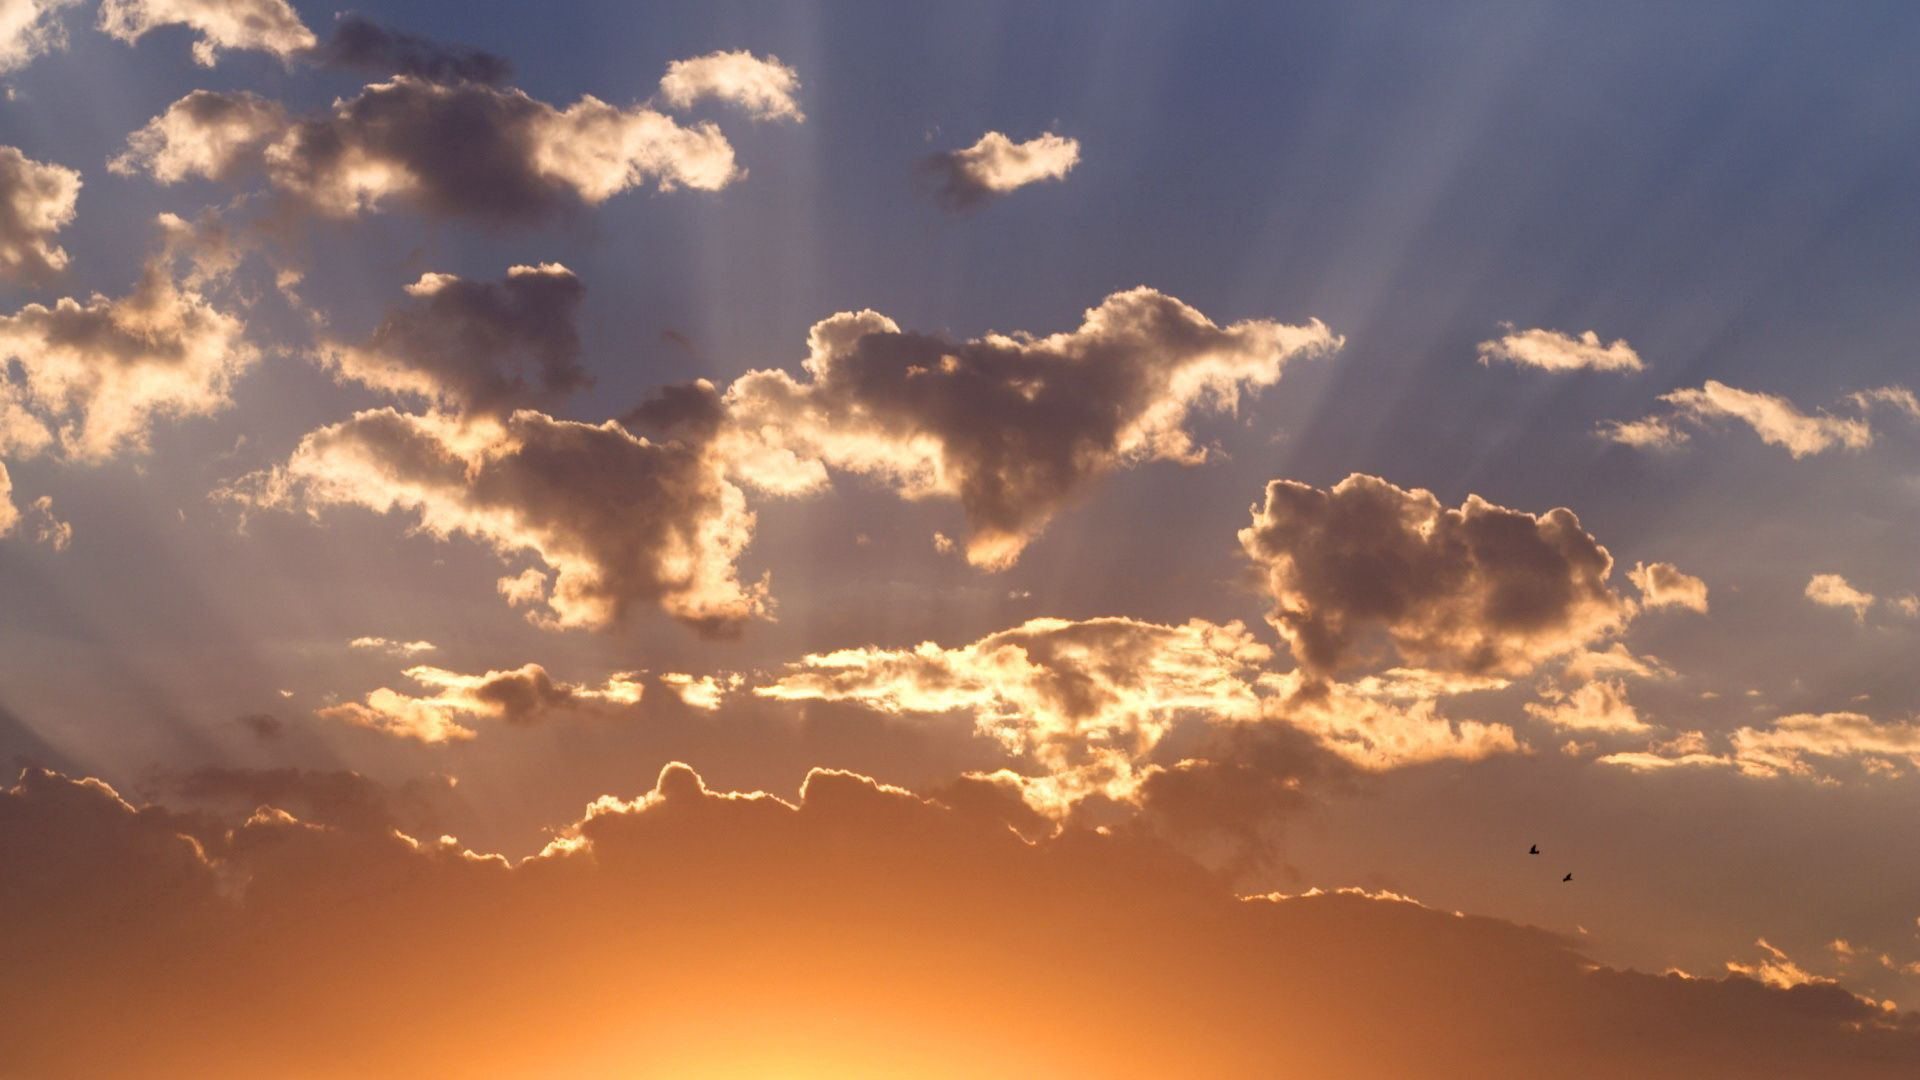
\includegraphics[scale=0.2]{sunset.jpg}
\centering
\label{fig:amanecer}
\caption*{Todos los derechos reservados a \maskCitet[p.2]{Diego2019}  o Elaboración propia}
\end{figure}




\begin{comment}
Incluir la figura en el documento "subiéndola" despues ejecutar: 
\begin{figure}[sentenciasA]
\includegraphics[sentenciasB]{nombreFigura.extensión}
% \centering o \raggedleft o \raggedright
\label{fig:nombreFigura}
\caption{Título de la figura, se incluye en el índice}
\caption*{Nota a la figura, derechos de autor, etc.}
\end{figure}

Sentencias A (posición):
    # h: por defecto, establece la posición de la figura justo despues del último elemento de la página.
    # t: figura al inicio de la página.
    # b: figura al final de la página.
    # p: inserta las figuras en una pagína por separado que solo contiene figuras.
    # !: inserta la figura en una posición "buena" de manera automática
    # H: la figura se coloca precisamente en el mismo lugar que aparece en el código.

Sentencias B (tamaño):
    # scale=X: X es igual a el porcentual que se desea de la figura, por ejemplo 0.5 es igual al el 50 porciento del tamaño de la figura.
    # width=\textwidth: ajusta el tamaño de la figura al tamaño del texto.
    
Referenciar figuras:
    # \ref{fig:nombreFigura} para mostrar el número de la figura
    # \pageref{fig:nombreFigura} para mostrar el número de página de la figura
\end{comment}
\newpage

\section{Tablas}
% https://www.tablesgenerator.com/#
% LAS MISMAS SENTENCIAS SE PUEDEN USAR EN TABLAS O CUADROS LAS REFERENCIAS INCLUSIVE
    % \ref{tab:my-tabledos}
\subsection{Título} 
Nunc ac consectetur elit. Vestibulum posuere venenatis dolor, ut scelerisque ligula porttitor a. Suspendisse potenti.\par
\begin{table}[h]
\centering
\caption{Mi Tabla}
\label{tab:my-tableuno}
\begin{tabular}{llllll}
\multicolumn{6}{c}{Letra x Fila} \\
A2  & B2  & C2  & D2  & E2  & F2 \\
A3  & B3  & C3  & D3  & E3  & F3 \\
A4  & B4  & C4  & D4  & E4  & F4 \\
A5  & B5  & C5  & D5  & E5  & F5
\end{tabular}
\caption*{Todos los derechos reservados a \maskCitet[p.2]{Diego2019}  o Elaboración propia}
\end{table}

\begin{table}[H]
\centering
\caption{Mi Segunda Tabla}

\label{tab:my-tabledos}
\begin{tabular}{|l|l|l|l|}
\hline
\multicolumn{4}{|c|}{\textbf{Colores}}                                                                                         \\ \hline
\multicolumn{1}{|c|}{\textit{X}} & \multicolumn{1}{c|}{\textit{Rojo}} & \multicolumn{1}{c|}{\textit{Azul}} & \textit{Amarillo} \\ \hline
\textit{Rojo}                    & {\ul Rojo}                         & Violeta                            & Naranja           \\ \hline
\textit{Azul}                    & Violeta                            & {\ul Azul}                         & Verde             \\ \hline
\textit{Amarillo}                & Naranja                            & Verde                              & {\ul Amarillo}    \\ \hline
\end{tabular}
\caption*{Todos los derechos reservados a \maskCitet[p.2]{Diego2019}  o Elaboración propia}
\end{table}






\newpage
% Referencias
\renewcommand\refname{\large\textbf{Referencias}}
\bibliography{mybibliography} % Se incluye el archivo mybibliography.bib
\begin{comment} % Sobre las referencias
# Se está usando "natbib"
# Se muestran únicamente las referencias usadas
\end{comment}

\end{document}